\chapter{Development of an Architectural Framework for a Distributed Cloud Manufacturing Platform in presence of autonomous nodes}
\section{Introduction}
This chapter presents the theoretical framework of this research in the form of a typical cloud manufacturing platform to investigate and explore cloud- resource sharing and execution of manufacturing process plans for heterogeneous decentralized autonomous manufacturing resources. The limitations identified in the previous chapter were used to develop a set of requirements and founding principles for the manufacturing systems.\\
Due to increasing globalization, manufacturing activities often require complex dynamics. Consequent design activities of manufacturing networks are useful in order to guarantee suitable decisions that could endure competition among companies. For this reason, product and process varieties are key factors to address customers' need for personalization, as well as strategies for companies. Phenomena connected to customers determine new factors that represent a challenge for industries, always ready to perform various manufacturing tasks within mass customization contexts. Indeed, modern manufacturing networks consist of suppliers that obey a unique principle: delivering products to the final customers belonging to the market. In such a context, smart technologies are essential in order to develop not- coupled and not-hierarchical heterogeneous systems, with the aim of satisfying constraints that, following needs of customizable products, market trends, and social media, allows directing expectations and desires, as well as demands of customers. In this direction, nowadays, an increasing necessity of personalized products is a growing necessity of international markets. This effort is the result of emerging mass customization that requires a fast and safe reconfiguration of various systems, especially of manufacturing type, as well as a competition that implies rapid changes in the customized production style.\\
Over the last few years, there has been a remarkable growth in the research activities related to the Industry 4.0 paradigm \parencite{zhou_industry_2015}. The term collectively refers to a wide range of technological concepts that provide solutions and advancement to different needs of manufacturing systems. Many smart manufacturing concepts and architecture have been proposed to bring higher flexibility with enhanced productivity, customization, and shortening the time to market. Combining emerging technologies with advanced manufacturing models, Cloud Manufacturing is a new manufacturing paradigm that meets the needs of manufacturing systems \parencite{kaynak_cloud_2020}.\\
In these models, resources are converted to independent and cooperative subsystems. These elements, connected to the physical environment through smart sensors, can work in Virtual Manufacturing Systems (VMS). A VMS is the aggregation and mapping of distributed physical elements. Each element may range across different levels of aggregation in the manufacturing processes from machine-level up to a whole production or logistics network.\\
Collectively seen, such new advances generate innovative technological possibilities potentially suitable to satisfy sophisticated customer demands, expectations, and desires. Building innovative models around the notion of being "globally virtual, locally physical" calls for a service-dominant logic of distributed resources in which reusable services models that represent homogeneous production processes are shaped according to the concept of Manufacturing as a Service \parencite{kayabay_wip_2018}.\\
A modern manufacturing network is composed of cooperating plants, suppliers, and dealers that produce and deliver final products to the market \parencite{mourtzis_design_2013}. These systems are no longer hierarchical physical and logical capsulated systems but heterogeneous, loosely coupled, non-hierarchical structured, cyber-physical systems of systems with event-based communication, collaboration in unified networks \parencite{nagorny_big_2017}. The idea of non-hierarchical production networks consisting of autonomous enterprises has been present in the scientific community for more than 20 years. Although current models, especially in large enterprises, are organizationally centralized due to size, need for control, and lack of third-party trust. It seems that this idea waited for production systems to acquire proper information and communications technology (ICT) or new industrial platforms, like Industry 4.0 \parencite{mladineo_solving_2017}. However, a strong effort towards Industry 4.0 is due to phenomena connected to Big-Data, also considering suitable ways by which industrial operations collect, manage and then interpret their own information \parencite{chen_data_2015}. This phenomenon is an obvious consequence of dynamics dealing with smart manufacturing systems, as they combine, mix and aggregate heterogeneous information sources located in different layers and/or domains. The possibility of achieving new status of associations, as well as finding patterns, is important within the context of Manufacturing for the reasons described as follows:
\begin{itemize}
    \item Criteria generation to construct decision systems for supply networks and manufacturing activities.
    \item Data continuous monitoring of fluctuations, with consequent predictions of future streams and their optimization.
\end{itemize}
Remarks and/or details about Big Data, as well as the analysis of datasets, are a challenge of each system within the Industry 4.0 environment. In this sense, conventional statistical processing approaches are not often useful because of the complexity and the size of large datasets. Actual implementations deal with adaptive scheduling, as well as a real-time modelling of processes and Decision Support Systems, useful to refine processes and design of components \parencite{oliff_towards_2017}. As for the context of logistics and production, a possible optimization foresees growth of resource efficiency \parencite{hauder_optimization_2017}. Such a situation allows the creation of different production technologies, with the consequent birth of new manufacturing models. The challenge with distributed production is to implement communication and integration technologies able to reduce the coordination effort and provide a focused factory \parencite{khajavi_additive_2014}.
\section{Main Assumptions and Founding Principles}
In the following scenario, the Cloud Manufacturing Network consists of nodes that utilize homogeneous technologies. These nodes are able to work in one or multiple distributed networks in an interoperable way. Each node inside the network can instance orders or buy production resources (slots) under the supervision of a coordinator that manages the negotiation and communication protocols among nodes.\\
Each network that works inside the platform follows three main principles: sustainability, transparency, and shared resources. In particular:
\begin{itemize}
    \item Sustainability deals with either reducing resource demands or CO2 emissions over the entire product life cycle that transfers the production closer to the client and with cost-effective manufacturing. In general, sustainability has not a definition of its own. However, there is consensus toward a research of compromises among resource and service needs, intending to guarantee either the satisfaction of users or the health of ecosystems that allows obtaining the resources.
    \item Transparency according to the Circular Economy trend, these networks need to create a transparent, collaborative, open, and trusting environment with shared purposes and resources.
    \item Shared resources refer to the possibility, for each node, to have equal unrestricted access to all possible resources inside the platform. Indeed, nodes can access other nodes’ resources through an open bidding system.
\end{itemize}

\section{Framework Components}
\subsection{Designing the architecture}
Architectures enable systems to operate and evolve, providing services inside an environment with a predictable level of quality, quantity, and performance. In operations management, architectures may present different definitions and scopes. Still, the core characteristic is concerned with providing a bridge between multiple system functionalities and requirements for defining the attributes that the system has to meet.\\
Distributed Manufacturing architectures have been thoroughly analyzed in academics and business fields. As a result, engineers have proposed different ways to reconfigure these systems with a common aim to expand functionalities and fulfill a broad range of requirements.\\
While there are still multiple definitions and architectures of Cloud Manufacturing, as depicted on Chapter II Section 2 and Section 3, a common objective is to connect end-users with a ubiquitous network domain of manufacturing service providers to enable co-creation \parencite{goran_advanced_2012}. The platform comprises multiple application layers responsible for service matching, manufacturing scheduling, optimization, and execution of the manufacturing process. Platform management is usually designed to be automated with centralized governance to provide efficient service coordination. In this case, the application layer can directly connect with a specific manufacturing provider obtaining information and making decisions through remote control of the specific resource.
\begin{figure}
    \centering
    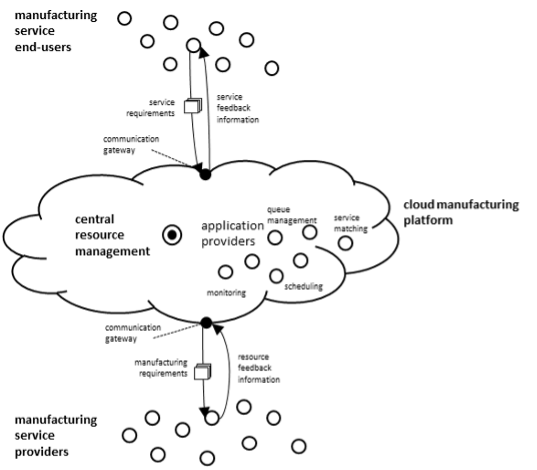
\includegraphics[height=4cm, keepaspectratio]{images/centralized-cmfg-architecture}
    \caption{Centralized Cloud Manufacturing Architecture}
    \label{fig:centralized-cmfg-architecture}
\end{figure}

A fully decentralized network architecture for cloud manufacturing (CMdna) has been proposed in \textcite{skulj_decentralised_2015}. In this work, the authors introduce a two layers architecture composed of an end-user layer and a service provider layer. This architecture presents fixed boundaries among layers and is based on Autonomous Work System (AWS). Most platform’s functionalities are decentralized to the AWS network distributing matching, scheduling, and decision-making mechanism among service providers.
\begin{figure}
    \centering
    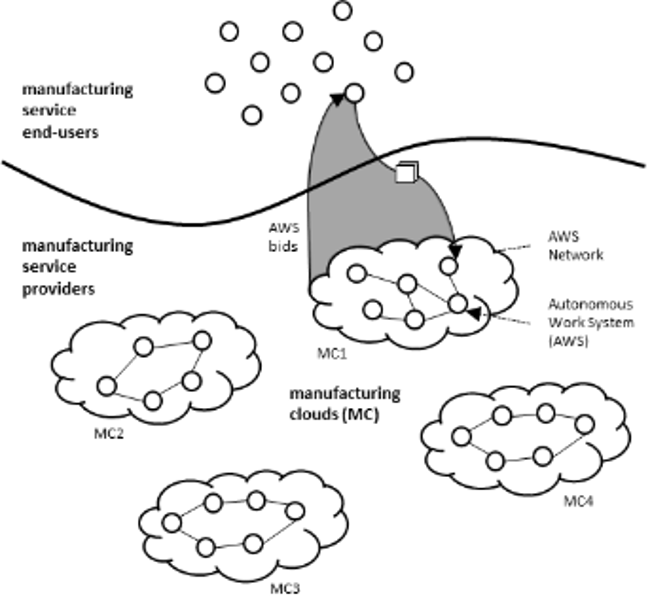
\includegraphics[height=4cm, keepaspectratio]{images/decentralized-cmfg-architecture}
    \caption{Decentralized Cloud Manufacturing Architecture}
    \label{fig:decentralized-cmfg-architecture}
\end{figure}

\subsection{Scattered Manufacturing Architecture}
In a Scattered Manufacturing platform, resources, labeled as nodes, can be either a service demander or a service provider. The coordination and the resource allocation process inside the network require a multi-stage negotiation activity among nodes and a platform agent. A global coordinator, called System Orchestrator (SO), is responsible for keeping platform operations aligned with Scattered Manufacturing founding principles (sustainability, equally shared resources, transparency) over time. Keeping the platform in line with its objectives over time, as market and technologies evolve, is a fundamental characteristic to keep robustness and flexibility.\\
In an Scattered Manufacturing architecture, decentralization occurs through service instantiation. After receiving multiple orders and applying the localization, filtering, and clustering algorithm, the Orchestrator needs to fragment the order into a finite number of tasks assigned to a subset of network resource providers. Each sub-network is an autonomous Virtual Manufacturing System (VMS) where a platform agent, Service Manager,negotiates resources with candidate manufacturing nodes through an opening bidding system. Each node is fully independent and may sell its manufacturing capacities to multiples sub-networks simultaneously or use their capacity for themselves. For better clarity, VMS are labeled as Services.
\begin{figure}
    \centering
    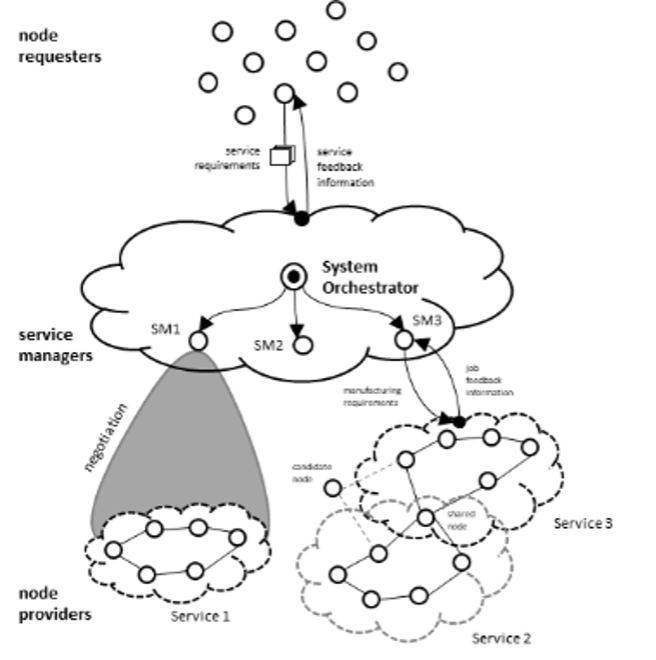
\includegraphics[height=4cm, keepaspectratio]{images/scattered-mfg-architecture}
    \caption{Scattered Manufacturing Architecture}
    \label{fig:smfg-architecture}
\end{figure}
\subsection{Cloud Manufacturing Architectures: a comparison}
Cloud Manufacturing architectures have similar advantages and disadvantages and reflect different needs from different physical systems. While Cloud Manufacturing's main strengths are efficiency and performance, it is also evident this platform can only be as flexible and robust as its centralized management. Scattered Manufacturing and Cloud Manufacturing Distributed network architecture present more flexibility in adapting to context and environment through a negotiation process from an architectural perspective.\\
Another difference among architectures is in their scope and size. While Cloud Manufacturing should be more suitable for Large Manufacturing Companies due to their characteristics, Scattered Manufacturing should fit more for Small and Medium Enterprises and micro-manufacturing networks. A comparison of the main characteristics and requirements of the three architectures is shown in Table 4.

\begin{table}
    \centering
    \begin{tabular}{|p{2.5cm}|p{2.5cm}|p{2.5cm}|p{2.5cm}|}
        \hline
        \textbf{Characteristic} & \textbf{CMfg} & \textbf{CMdna} & \textbf{SMfg} \\
        \hline
        No. of layers & users (consumers), application providers, physical resource providers & service users, service providers & system orchestrator, service managers, service nodes \\
        \hline
        Physical resource providers & Third-party or platform owned & AWSs & Associated autonomous nodes\\ 
        \hline
        End-users & External user & External user & Internal or External node/users\\
        \hline
        Resource Management & centralized within CM platform & decentralized to AWS level & decentralized to Node level\\ 
        \hline
        Service Matching & Application providers & End-Users & Service Agent\\
        \hline
        Resource allocation & Direct allocation & Asynchronously through propagation & Negotiation among a service manager and candidates nodes\\
        \hline
        Information flow & Vertical & Horizontal & Vertical and Horizontal\\
        \hline
        Scheduling & Centralized, developed by an application provider & Provided by the end-user & Developed by service managers coordinated by an Orchestrator\\
        \hline
        Optimization size & Global optimization & Local optimization, no virtual coordinator & Local optimization (SM)\\
        \hline
        Optimization scope & Short and medium term & Short-term & Global optimization (SO) Short-term (SM) Medium-long term (SO)\\
        \hline 
    \end{tabular}

    \caption{A comparison among network architectures}
    \label{tab:architectures-comparison}
\end{table}
Finally, because of their structure, decentralized solutions may present drawbacks due to the higher degree of complexity and coordination needed:
\begin{itemize}
    \item The platform must deal with the additional complexity and overheads from the granular nature of a distributed system based on autonomous resources.
    \item Current architectures are mainly oriented on building a monolithic Cloud Manufacturing platform with fully managed nodes to simplify the master planning and monitoring process.
    \item Monitoring Key Performance Indicators is a more complex process due to the need for monitoring globally distributed autonomous physical resources.
    \item Architects and engineers need to implement an intra-service formal negotiation mechanism and communication protocol.
    \item Communication protocols should also be able to support effective interactions among Service Agents and Node Managers.
    \item Implementing processes that span limited resources across multiple services without global coordination is challenging.
    \item The architecture requires careful coordination among services.
    \item Deployment complexity. There is also a computational complexity of the software needed to deploy multiple agents and manage a system comprised of many different services simultaneously.
\end{itemize}

\section{Building the platform model}
This section defines the layout, agents, and functionalities for the Scattered Manufacturing platform. The three building blocks of the platform are (i) Architecture, (ii) Actors/Structure/Functions, (iii) Founding Principles.
\begin{figure}[h]
    \centering
    
\includegraphics[height=4cm, keepaspectratio]{images/platform-building-blocks}
    \caption{Platform Building Blocks}
    \label{fig:platform-building-blocks}
\end{figure}
We can classify the main functionalities of this platform as follows:
\begin{enumerate}
    \item Service Transactions Management: ordering, negotiation, contracting, delivering, payments.
    \item Platform Operations Coordination: automated order processing, order decomposition, demand matching, load balance, job composition, task composition, platform, and service schedule.
    \item Monitoring: concerning three different dimensions; (a) size (orders, job, task); (b) scope (global, service, local), (c) level of aggregation (i) Platform monitoring (ii) Service Monitoring (iii) Node Monitoring.
    \item Evolution: adaptation of tactics and strategies used by the System Orchestrator, Service Coordinator, and Node Manager based on a continuous learning process.
\end{enumerate}
The first two functionalities refer to the need for managing and operating a manufacturing and logistics network. A first assumption is that every node inside the network has been vetted with a preliminary registration process to parametrize different aspects of the process, such as orders generation, contracting, payment transactions, logistics, a messaging protocol for the open bidding system, and reporting and analytics protocol. Another assumption is that each order is composed of independent jobs that can be split and rearrange in tasks without logical dependencies.
Other functional features inside the network are classified in Table \ref{tab:platform-functional-features}:
\begin{table}
    \centering
    \begin{tabular}{|p{3cm}|p{6cm}|}
        \hline
        \textbf{Features} & \textbf{Description}\\
        \hline
        Jobs Generation & Processing, filtering, and automated clustering of incoming orders based on selective and relevant features \\
        \hline
        Service instantiation & Instantiation of a new service to process and deliver a Job. A Service can be defined as a Virtual Manufacturing System (VMS). At the end of the negotiation process, the VMS negotiates capacity and prices and determines the schedule allocating a set of tasks to selected nodes. After concluding the job, the service and the related VMS terminates, and the nodes rearrange in new services bidding for new orders.\\
        \hline
        Service negotiation & Automated negotiation system based on software agents. representing the Service Coordinator, responsible for meeting jobs requirements and resource offerings, and the Node Managers, responsible for the machines scheduling and operations pursuing node objectives\\
        \hline
        Real-time scheduling and planning & Service Coordinators continuously send feedback about their jobs to the System Orchestrator. Based on the information received, the S.O. adapt the master planning, changing its strategy when instantiating new services\\
        \hline
    \end{tabular}
    \caption{Platform Functional Features}
    \label{tab:platform-functional-features}
\end{table}
\subsection{Platform Structure}
Nodes inside the network can issue orders or sell production slots. An orchestrator determines the dynamics along with the network, managing communication activities among nodes via principles of equated shared resources, sustainability, and transparency. A unique approach is helpful to establish tradeoffs for the characterization of logistics and production costs in terms of resource allocation and show negotiation criteria among nodes. As for picking activities, the Author has proposed, on Chapter IV Section 3 Paragraph vi, a multi-stage algorithm that, once origins and destination are fixed, finds the route that permits to reach the destination in the shortest time.\\
Load balancing represents one of the key features to reach an equilibrium inside the network. Load Balance can be seen as the platform mechanism for self-regulation. Load Balance refers to the process of distributing a set of tasks over a set of resources to make their overall process more efficient. Load balancing can optimize the response time and avoid unevenly overloading some nodes while other resources are left idle. Different levels of load balance occur in the platform to reach an equilibrium in the overall network and in each service. A global load balancer should also implement a failover for those services that become non-responsive in allocating new jobs. This feature needs continuous monitoring through feedback communication systems from different levels of the network, such as Service Coordinators and Node Managers. In those cases, the System Orchestrator stops sending Jobs to that area of the network, instantiating new services in different regions or widening the size of the network that the service should query.\\
Another critical functionality to build a dynamic and stable open distributed network is the ability to instantiate new manufacturing networks when a service is needed. A Virtual Manufacturing System (VMS) is a key piece of a Scattered Manufacturing architecture. It can be defined as an ephemeral manufacturing system with variable dimensions and localization that dynamically changes its topology with time and scope. A VMS is deployed as a service each time the System Orchestrator needs to launch a new Job. Once the job is effectively delivered, the network and the relationships within its nodes are terminated. VMS introduces the ability of large-scale parallelism, and it is designed explicitly for a market-driven supply chain that requires carrying out lightweight network infrastructure and fast processing time in response to highly varying market needs. Indeed, the service can be seen as an operations function triggered when there is an actual market need. The networkless system can potentially become more adaptive, flexible, and efficient than traditional networks. This approach is location independent and, combined with fast, focused local area suppliers, could lead to better performance and scalability. Further, because every node inside the network can operate without the entry barrier of building and maintain a large supply chain infrastructure and working on its coordination, each node can focus more on the reliability and quality of the production.
\subsection{Platform Functionalities}
When the S.O. receives orders from multiple sources (external and internal associated nodes), it starts scanning the status of deployed services, and it assesses the overall platform load balance. Then it initiates the automated filtering and clustering algorithm that uses relevant features to decompose orders into jobs. After determining the size and localization of the service, the S.O. registers a new service deploying it inside the platform. Each service is initiated with Job characteristics and a first attempt of the network topology. This phase aims to reduce the manufacturing and logistics costs associated with a specific Job by searching and selecting candidate nodes. Once deployed, the S.O. leaves the service coordination to S.C.. Then, S.C. starts the multi-stage negotiation process with candidate nodes with a first attempt at balancing prices and workloads. At this stage, each node will deploy its strategies. In particular, it is worth mentioning that each node may not wish to subordinate their capacity to a specific service entirely, or they can probably also operate outside the platform. The presence of a service coordinator that needs to negotiate capacities and task prices with cooperative and competitive nodes ensures the balance is reached by the agents involved. Based on the response of the current negotiation iteration, S.C. has three possible actions to undertake:
\begin{enumerate}
    \item In case of partial consensus, adapt the planning based on the feedback received from the nodes.
    \item In case of total agreement, launch the task scheduler to initiate the service.
    \item If the number of negotiation cycles is higher than a threshold iterations parameter, S.C. sends a denial of service message to the S.O.. In that case, the Job returns into the order pool and is managed by the S.O.. Based on the analysis of the states and actions previously taken, the System Orchestrator triggers a new deployment plan for the Job.
\end{enumerate}

\begin{figure}[h]
    \centering
    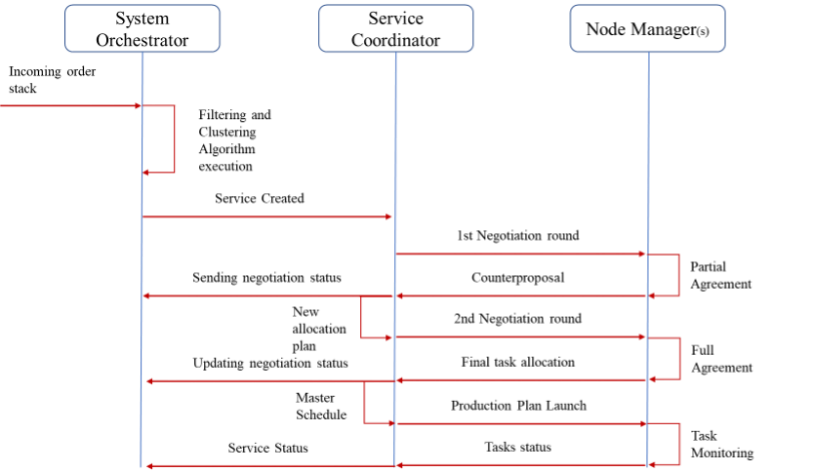
\includegraphics[height=4cm, keepaspectratio]{images/operations-mode-smfg}
    \caption{Operations mode of the SMfg platform}
    \label{fig:operations-mode-smfg}
\end{figure}

\subsection{Platform Coordination and Negotiation Mechanisms}
In such a distributed and opened system, coordination ensures that autonomous agents can act in a tightly coordinated manner to effectively reach their goals. This matter can be addressed, at least in part, by designing agents that communicate and cooperate through negotiation. The negotiation process is a sophisticated feature for introducing flexibility, efficiency, and achieving coordination in an open distributed manufacturing system.\\
Coordination mechanisms of actors involved should rely on decentralized governance to create an ecosystem-wide intelligence for adaptive control of platform operations. While centralized governance need of command-and- control poses potential issues in terms of the system’s flexibility and scalability \parencite{putnik_scalability_2013}, decentralization of manufacturing system governance introduces structural complexity. The model requires to fully absorb the increased intricacies, variety of variables, and objectives of a modern manufacturing system. Therefore, a viable approach is the decomposition of decision-making tasks to improve the model's capability to understand and generalize complexity. In order to manage uncertainty and volatile dynamics, the model needs to introduce a certain degree of automation in decision-making and governance processes. Since it is impossible to model and rationalize each state and dynamic, advanced machine learning techniques are required. The model should be affected by the underlying system evolution and the decisions made by other autonomous elements, who are concurrently improving their policies through continuous learning. Continuous learning could be achieved with automated negotiation systems where software agents representing individuals or organizations are capable of reaching an agreement. This topic has seen a great deal of attention in the last decade from Multi-Agent Systems to Machine Learning and Artificial Intelligence researchers and represents a potential solution in simulating these systems \parencite{lopes_negotiation_2009}.\\
Modeling mechanisms of coordination and dynamics in the behavior of each entity inside the network requires a good reasoning capacity about the long-term consequences of actions taken \parencite{guizzi_integrating_2013}. Configuring and managing strategies and tactics of each entity with an evolutionary approach is the main challenge for these systems. For example, as described in \textcite{haj2019view}, a good job scheduler that should manage and interact within a cloud manufacturing sub-network should make decisions that are either reasonable for the immediate reward and good in the long term the sustainability of the network. Such an agent should sometimes forget short-term objectives in a shared effort of realizing greater long-term benefits. The scheduler agent should also adapt and react to variations in the underlying resource performance and scale in the presence of new or unseen workloads combined with large numbers of resources. Another fundamental requirement is model scalability and reconfigurability \parencite{putnik_scalability_2013}. Indeed, the system should require a good generalization capacity, letting agents adapt to new environments, and the ability to decide in states of the environment that the model has not previously seen.
